\documentclass{beamer}

\usepackage{subcaption}
\usepackage{graphicx}
\usepackage{tikz}

\author{Manuel Frohn}
\title{Planare Graphen - Coloring}
\institute{RWTH Aachen University, Aachen, Germany}
\date{?}

\begin{document}
    \begin{frame}
        \maketitle
    \end{frame}

    \begin{frame}
        \frametitle{Inhaltsverzeichnis}
        \tableofcontents
    \end{frame}

    \section{Relevanz}

    \begin{frame}
        \frametitle{Relevanz}
        \begin{enumerate}
            \item Real auftretene Klasse
            \item Wichtig für Chip Design
            \item Bedingung für Algorithmen und Sätze
            \item Zuweisungsprobleme als Coloring
        \end{enumerate}
    \end{frame}

    \section{Planare Graphen}
    \subsection{Einführung}

    \begin{frame}
        \frametitle{Planare Graphen}
        \begin{definition}[Planarität]
            Ein Graph G heißt planar, wenn man in der Lage
            ist, den Graphen so auf eine Ebene zu zeichnen, dass sich seine Kanten nicht
            schneiden.          
        \end{definition}
    \end{frame}
    
    \begin{frame}
        \frametitle{Planare Graphen Beispiel}
        \begin{figure}
            \begin{subfigure}{.33\textwidth}
                \centering
                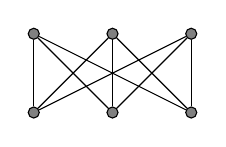
\begin{tikzpicture}[every node/.style={circle, draw, fill=black!50,inner sep=0pt, minimum width=4pt},
                    edge_style/.style={draw=black}]
                    \node (v1) at (0, 0) {};
                    \node (v2) at (1, 0) {};
                    \node (v3) at (2, 0) {};
                    \node (v4) at (0, 1) {};
                    \node (v5) at (1, 1) {};
                    \node (v6) at (2, 1) {};  
                    \draw (v1) edge (v4);
                    \draw (v1) edge (v5);
                    \draw (v1) edge (v6);
                    \draw (v2) edge (v4);
                    \draw (v2) edge (v5);
                    \draw (v2) edge (v6);
                    \draw (v3) edge (v4);
                    \draw (v3) edge (v5);
                    \draw (v3) edge (v6);
                \end{tikzpicture}
                \caption{$K_{3,3}$}
            \end{subfigure}
            \begin{subfigure}{.33\textwidth}
                \centering
                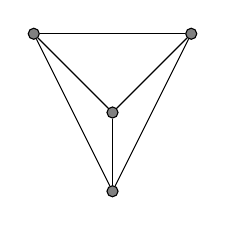
\begin{tikzpicture}[every node/.style={circle, draw, fill=black!50,inner sep=0pt, minimum width=4pt},
                    edge_style/.style={draw=black}]
                    \node (v1) at (1, 0) {};
                    \node (v2) at (1, 1) {};
                    \node (v3) at (0, 2) {};
                    \node (v4) at (2, 2) {};
                    \draw (v1) edge (v2);
                    \draw (v1) edge (v3);
                    \draw (v1) edge (v4);
                    \draw (v2) edge (v3);
                    \draw (v2) edge (v4);
                    \draw (v4) edge (v3);
                \end{tikzpicture}
                \caption{$K_4$}
            \end{subfigure}
            \begin{subfigure}{.30\textwidth}
                \centering
                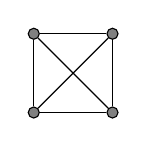
\begin{tikzpicture}[every node/.style={circle, draw, fill=black!50,inner sep=0pt, minimum width=4pt},
                    edge_style/.style={draw=black}]
                    \node (v1) at (0, 0) {};
                    \node (v2) at (0, 1) {};
                    \node (v3) at (1, 0) {};
                    \node (v4) at (1, 1) {};
                    \draw (v1) edge (v2);
                    \draw (v1) edge (v3);
                    \draw (v1) edge (v4);
                    \draw (v2) edge (v3);
                    \draw (v2) edge (v4);
                    \draw (v4) edge (v3);
                \end{tikzpicture}
                \caption{$K_4$}
            \end{subfigure}
        \end{figure}
    \end{frame}

    \subsection{Exkurs: Minore}
    \begin{frame}
        \frametitle{Minor}
        \begin{definition}
            M heißt Minor von G wenn M aus einem Teilgarphen
            von G, durch Kantenkontaktion hervorgeht.
        \end{definition}
        \begin{figure}
            \begin{subfigure}{.50\textwidth}
                \centering
                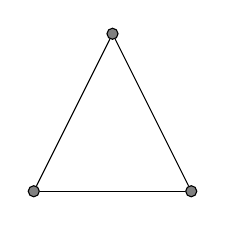
\begin{tikzpicture} [every node/.style={circle, draw, fill=black!50,inner sep=0pt, minimum width=4pt},
                    edge_style/.style={draw=black}]
                    \node (v1) at (0,0) {};
                    \node (v2) at (2,0) {};
                    \node (v3) at (1,2) {};
                    \draw (v1) edge (v2) {};
                    \draw (v2) edge (v3) {};
                    \draw (v3) edge (v1) {};
                \end{tikzpicture}
            \end{subfigure}
            \begin{subfigure}{.48\textwidth}
                \centering
                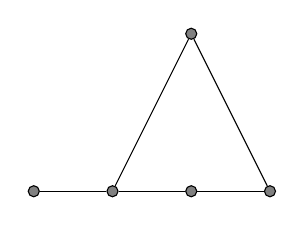
\begin{tikzpicture} [every node/.style={circle, draw, fill=black!50,inner sep=0pt, minimum width=4pt},
                    edge_style/.style={draw=black}]
                    \node (v1) at (0,0) {};
                    \node (v2) at (1,0) {};
                    \node (v3) at (2,0) {};
                    \node (v4) at (3,0) {};
                    \node (v5) at (2,2) {};
                    \draw (v1) edge (v2) {};
                    \draw (v2) edge (v3) {};
                    \draw (v3) edge (v4) {};
                    \draw (v4) edge (v5) {};
                    \draw (v2) edge (v5) {};
                \end{tikzpicture}
            \end{subfigure}
        \end{figure}
    \end{frame}

    \begin{frame}
        \frametitle{Kantenkontraktion}
        \begin{definition}[Kantenkontraktion]
            Gegeben ein Graph $G = (V,E)$ und eine Kante $ e = {v, w} \in E $, ist das Resultat der Kontraktion von e, der Graph $G' = (V', E')$ mit
            $V' = (V \setminus e) \cup \{n \}$ und $E' = (E \setminus \{v \in e \lor w \in e  \mid e \in E \}) \cup \{ \{n, z\} \mid z,v \in e \in E \lor z,w \in e \in E\}$
        \end{definition}
    \end{frame}

    \begin{frame}
        \frametitle{Kantenkontraktion Beispiel}
        \centering
        \only<1>{
            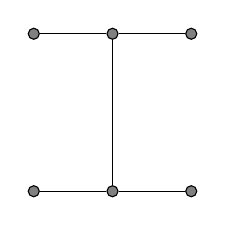
\begin{tikzpicture}[every node/.style={circle, draw, fill=black!50,inner sep=0pt, minimum width=4pt},
                edge_style/.style={draw=black}]
                \node (v1) at (0, 0) {};
                \node (v2) at (1, 0) {};
                \node (v3) at (2, 0) {};
                \node (v4) at (0, 2) {};
                \node (v5) at (1, 2) {};
                \node (v6) at (2, 2) {};
                \draw (v1) edge (v2) {};
                \draw (v2) edge (v3) {};
                \draw (v2) edge (v5) {};
                \draw (v4) edge (v5) {};
                \draw (v5) edge (v6) {};
            \end{tikzpicture}
        }
        \only<2>{
            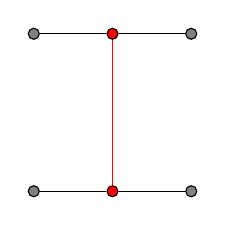
\begin{tikzpicture}[every node/.style={circle, draw, fill=black!50,inner sep=0pt, minimum width=4pt},
                edge_style/.style={draw=black}]
                \tikzset{red edge/.style={draw=red}}
                \tikzset{red node/.style={fill=red}}
                \node (v1) at (0, 0) {};
                \node [red node] (v2) at (1, 0) {};
                \node (v3) at (2, 0) {};
                \node (v4) at (0, 2) {};
                \node [red node] (v5) at (1, 2) {};
                \node (v6) at (2, 2) {};
                \draw (v1) edge (v2) {};
                \draw (v2) edge (v3) {};
                \draw[red edge] (v2) edge (v5) {};
                \draw (v4) edge (v5) {};
                \draw (v5) edge (v6) {};
            \end{tikzpicture}
        }
        \only<3>{
            \begin{tikzpicture}[every node/.style={circle, draw, fill=black!50,inner sep=0pt, minimum width=4pt},
                edge_style/.style={draw=black}]
                \tikzset{green node/.style={fill=green}}
                \node (v1) at (0, 0) {};
                \node (v3) at (2, 0) {};
                \node (v4) at (0, 2) {};
                \node (v6) at (2, 2) {};
                \node [green node] (vn) at (1, 1) {};
                \draw (v1) edge (v2) {};
                \draw (v2) edge (v3) {};
                \draw (v4) edge (v5) {};
                \draw (v5) edge (v6) {};
            \end{tikzpicture}
        }
        \only<4>{
            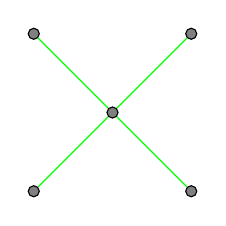
\begin{tikzpicture}[every node/.style={circle, draw, fill=black!50,inner sep=0pt, minimum width=4pt},
                edge_style/.style={draw=black}]
                \tikzset{green edge/.style={draw=green}}
                \node (v1) at (0, 0) {};
                \node (vn) at (1, 1) {};
                \node (v3) at (2, 0) {};
                \node (v4) at (0, 2) {};
                \node (v6) at (2, 2) {};
                \draw [green edge] (v1) edge (vn) {};
                \draw [green edge] (v3) edge (vn) {};
                \draw [green edge] (v4) edge (vn) {};
                \draw [green edge] (v6) edge (vn) {};
            \end{tikzpicture}
        }
        \only<5>{
            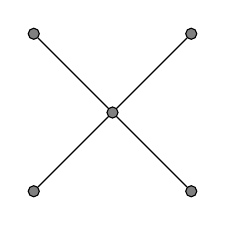
\begin{tikzpicture}[every node/.style={circle, draw, fill=black!50,inner sep=0pt, minimum width=4pt},
                edge_style/.style={draw=black}]
                \node (v1) at (0, 0) {};
                \node (vn) at (1, 1) {};
                \node (v3) at (2, 0) {};
                \node (v4) at (0, 2) {};
                \node (v6) at (2, 2) {};
                \draw (v1) edge (vn) {};
                \draw (v3) edge (vn) {};
                \draw (v4) edge (vn) {};
                \draw (v6) edge (vn) {};
            \end{tikzpicture}
        }
    \end{frame}

    \begin{frame}
        \frametitle{Minor Beispiel}
        \centering
        \only<1>{
            \centering
            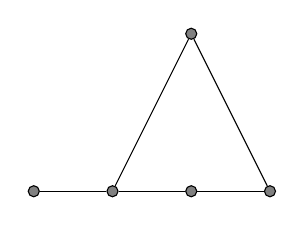
\begin{tikzpicture} [every node/.style={circle, draw, fill=black!50,inner sep=0pt, minimum width=4pt},
                edge_style/.style={draw=black}]
                \node (v1) at (0,0) {};
                \node (v2) at (1,0) {};
                \node (v3) at (2,0) {};
                \node (v4) at (3,0) {};
                \node (v5) at (2,2) {};
                \draw (v1) edge (v2) {};
                \draw (v2) edge (v3) {};
                \draw (v3) edge (v4) {};
                \draw (v4) edge (v5) {};
                \draw (v2) edge (v5) {};
            \end{tikzpicture} 
        }
        \only<2>{
            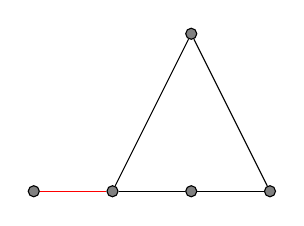
\begin{tikzpicture} [every node/.style={circle, draw, fill=black!50,inner sep=0pt, minimum width=4pt},
                edge_style/.style={draw=black}]
                \tikzset{red edge/.style={draw=red}}
                \node (v1) at (0,0) {};
                \node (v2) at (1,0) {};
                \node (v3) at (2,0) {};
                \node (v4) at (3,0) {};
                \node (v5) at (2,2) {};
                \draw [red edge] (v1) edge (v2) {};
                \draw (v2) edge (v3) {};
                \draw (v3) edge (v4) {};
                \draw (v4) edge (v5) {};
                \draw (v2) edge (v5) {};
            \end{tikzpicture} 
        }
        \only<3>{
            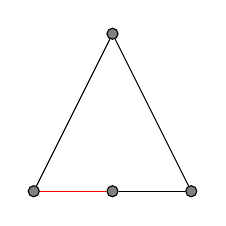
\begin{tikzpicture} [every node/.style={circle, draw, fill=black!50,inner sep=0pt, minimum width=4pt},
                edge_style/.style={draw=black}]
                \tikzset{red edge/.style={draw=red}}
                \node (v2) at (1,0) {};
                \node (v3) at (2,0) {};
                \node (v4) at (3,0) {};
                \node (v5) at (2,2) {};
                \draw [red edge] (v2) edge (v3) {};
                \draw (v3) edge (v4) {};
                \draw (v4) edge (v5) {};
                \draw (v2) edge (v5) {};
            \end{tikzpicture} 
        }
        \only<4>{
            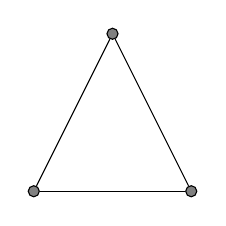
\begin{tikzpicture} [every node/.style={circle, draw, fill=black!50,inner sep=0pt, minimum width=4pt},
                edge_style/.style={draw=black}]
                \tikzset{red edge/.style={draw=red}}
                \node (v2) at (1,0) {};
                \node (v4) at (3,0) {};
                \node (v5) at (2,2) {};
                \draw (v2) edge (v4) {};
                \draw (v4) edge (v5) {};
                \draw (v2) edge (v5) {};
            \end{tikzpicture} 
        }
    \end{frame}

    \subsection{Wichtige Sätze}
    \begin{frame}
        \frametitle{Eulerscher Polyedersatz}
        \visible<1->{
            \begin{Satz}
                Gegeben ein planarer Graph G = (V, E) und die Anzahl seiner Gebiete $|G|$ gilt: $|V| - |E| + |G| = 2$
            \end{Satz}
        }
        \visible<2>{
            \begin{Satz}
                $G$ Planar $ \Leftrightarrow |E| \leq 3|V| - 6 \land |G| \leq 2|V| - 4$
            \end{Satz}
        }
        
    \end{frame}

    \begin{frame}
        \frametitle{Gebiete}
        \centering
        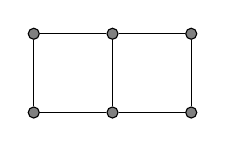
\begin{tikzpicture}[every node/.style={circle, draw, fill=black!50,inner sep=0pt, minimum width=4pt},
            edge_style/.style={draw=black}]
            \node (v1) at (0,0){};
            \node (v2) at (0,1){};
            \node (v3) at (1,0){};
            \node (v4) at (1,1){};
            \node (v5) at (2,0){};
            \node (v6) at (2,1){};
            \draw (v1) edge (v2);
            \draw (v2) edge (v4);
            \draw (v4) edge (v6);
            \draw (v5) edge (v6);
            \draw (v3) edge (v4);
            \draw (v1) edge (v3);
            \draw (v3) edge (v5);
        \end{tikzpicture}
    \end{frame}

    \begin{frame}
        \frametitle{Satz von Kuratowski}
        \begin{Satz}
            Ein Graph ist genau dann planar, wenn er weder den $K{3,3}$ noch den $K_5$ als Minor enthält
        \end{Satz}
        \begin{figure}
            \begin{subfigure}{.50\textwidth}
                \centering
                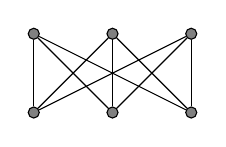
\begin{tikzpicture}[every node/.style={circle, draw, fill=black!50,inner sep=0pt, minimum width=4pt},
                    edge_style/.style={draw=black}]
                    \node (v1) at (0, 0) {};
                    \node (v2) at (1, 0) {};
                    \node (v3) at (2, 0) {};
                    \node (v4) at (0, 1) {};
                    \node (v5) at (1, 1) {};
                    \node (v6) at (2, 1) {};  
                    \draw (v1) edge (v4);
                    \draw (v1) edge (v5);
                    \draw (v1) edge (v6);
                    \draw (v2) edge (v4);
                    \draw (v2) edge (v5);
                    \draw (v2) edge (v6);
                    \draw (v3) edge (v4);
                    \draw (v3) edge (v5);
                    \draw (v3) edge (v6);
                \end{tikzpicture}
                \caption{$K_{3,3}$}
            \end{subfigure}
            \begin{subfigure}{.48\textwidth}
                \centering
                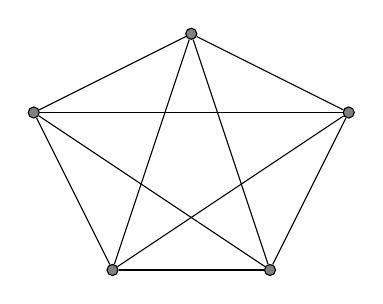
\begin{tikzpicture}[every node/.style={circle, draw, fill=black!50,inner sep=0pt, minimum width=4pt},
                    edge_style/.style={draw=black}]
                    \node (v1) at (1, 0) {};
                    \node (v2) at (3, 0) {};
                    \node (v3) at (0, 2) {};
                    \node (v4) at (4, 2) {};
                    \node (v5) at (2, 3) {};
                    \draw (v1) edge (v2);
                    \draw (v1) edge (v3);
                    \draw (v1) edge (v4);
                    \draw (v1) edge (v5);
                    \draw (v2) edge (v3);
                    \draw (v2) edge (v4);
                    \draw (v2) edge (v5);
                    \draw (v3) edge (v4);
                    \draw (v3) edge (v5);
                    \draw (v4) edge (v5);
                \end{tikzpicture}
                \caption{$K_5$}
            \end{subfigure}
        \end{figure}
    \end{frame}
\end{document}